
%% bare_conf.tex
%% V1.4b
%% 2015/08/26
%% by Michael Shell
%% See:
%% http://www.michaelshell.org/
%% for current contact information.
%%
%% This is a skeleton file demonstrating the use of IEEEtran.cls
%% (requires IEEEtran.cls version 1.8b or later) with an IEEE
%% conference paper.
%%
%% Support sites:
%% http://www.michaelshell.org/tex/ieeetran/
%% http://www.ctan.org/pkg/ieeetran
%% and
%% http://www.ieee.org/

%%*************************************************************************
%% Legal Notice:
%% This code is offered as-is without any warranty either expressed or
%% implied; without even the implied warranty of MERCHANTABILITY or
%% FITNESS FOR A PARTICULAR PURPOSE! 
%% User assumes all risk.
%% In no event shall the IEEE or any contributor to this code be liable for
%% any damages or losses, including, but not limited to, incidental,
%% consequential, or any other damages, resulting from the use or misuse
%% of any information contained here.
%%
%% All comments are the opinions of their respective authors and are not
%% necessarily endorsed by the IEEE.
%%
%% This work is distributed under the LaTeX Project Public License (LPPL)
%% ( http://www.latex-project.org/ ) version 1.3, and may be freely used,
%% distributed and modified. A copy of the LPPL, version 1.3, is included
%% in the base LaTeX documentation of all distributions of LaTeX released
%% 2003/12/01 or later.
%% Retain all contribution notices and credits.
%% ** Modified files should be clearly indicated as such, including  **
%% ** renaming them and changing author support contact information. **
%%*************************************************************************


% *** Authors should verify (and, if needed, correct) their LaTeX system  ***
% *** with the testflow diagnostic prior to trusting their LaTeX platform ***
% *** with production work. The IEEE's font choices and paper sizes can   ***
% *** trigger bugs that do not appear when using other class files.       ***                          ***
% The testflow support page is at:
% http://www.michaelshell.org/tex/testflow/



\documentclass[conference]{IEEEtran}
% Some Computer Society conferences also require the compsoc mode option,
% but others use the standard conference format.
%
% If IEEEtran.cls has not been installed into the LaTeX system files,
% manually specify the path to it like:
% \documentclass[conference]{../sty/IEEEtran}





% Some very useful LaTeX packages include:
% (uncomment the ones you want to load)


% *** MISC UTILITY PACKAGES ***
%
%\usepackage{ifpdf}
% Heiko Oberdiek's ifpdf.sty is very useful if you need conditional
% compilation based on whether the output is pdf or dvi.
% usage:
% \ifpdf
%   % pdf code
% \else
%   % dvi code
% \fi
% The latest version of ifpdf.sty can be obtained from:
% http://www.ctan.org/pkg/ifpdf
% Also, note that IEEEtran.cls V1.7 and later provides a builtin
% \ifCLASSINFOpdf conditional that works the same way.
% When switching from latex to pdflatex and vice-versa, the compiler may
% have to be run twice to clear warning/error messages.






% *** CITATION PACKAGES ***
%
%\usepackage{cite}
% cite.sty was written by Donald Arseneau
% V1.6 and later of IEEEtran pre-defines the format of the cite.sty package
% \cite{} output to follow that of the IEEE. Loading the cite package will
% result in citation numbers being automatically sorted and properly
% "compressed/ranged". e.g., [1], [9], [2], [7], [5], [6] without using
% cite.sty will become [1], [2], [5]--[7], [9] using cite.sty. cite.sty's
% \cite will automatically add leading space, if needed. Use cite.sty's
% noadjust option (cite.sty V3.8 and later) if you want to turn this off
% such as if a citation ever needs to be enclosed in parenthesis.
% cite.sty is already installed on most LaTeX systems. Be sure and use
% version 5.0 (2009-03-20) and later if using hyperref.sty.
% The latest version can be obtained at:
% http://www.ctan.org/pkg/cite
% The documentation is contained in the cite.sty file itself.






% *** GRAPHICS RELATED PACKAGES ***
%
\ifCLASSINFOpdf
   \usepackage[pdftex]{graphicx}
  % declare the path(s) where your graphic files are
   \graphicspath{{C:/Users/chuprina/Documents/PhD/Conferences/RE/2018/IEEEtran/pictures/}}
  % and their extensions so you won't have to specify these with
  % every instance of \includegraphics
  \DeclareGraphicsExtensions{.pdf,.jpeg,.png}
\else
  % or other class option (dvipsone, dvipdf, if not using dvips). graphicx
  % will default to the driver specified in the system graphics.cfg if no
  % driver is specified.
  % \usepackage[dvips]{graphicx}
  % declare the path(s) where your graphic files are
  % \graphicspath{{../eps/}}
  % and their extensions so you won't have to specify these with
  % every instance of \includegraphics
  % \DeclareGraphicsExtensions{.eps}
\fi
% graphicx was written by David Carlisle and Sebastian Rahtz. It is
% required if you want graphics, photos, etc. graphicx.sty is already
% installed on most LaTeX systems. The latest version and documentation
% can be obtained at: 
% http://www.ctan.org/pkg/graphicx
% Another good source of documentation is "Using Imported Graphics in
% LaTeX2e" by Keith Reckdahl which can be found at:
% http://www.ctan.org/pkg/epslatex
%
% latex, and pdflatex in dvi mode, support graphics in encapsulated
% postscript (.eps) format. pdflatex in pdf mode supports graphics
% in .pdf, .jpeg, .png and .mps (metapost) formats. Users should ensure
% that all non-photo figures use a vector format (.eps, .pdf, .mps) and
% not a bitmapped formats (.jpeg, .png). The IEEE frowns on bitmapped formats
% which can result in "jaggedy"/blurry rendering of lines and letters as
% well as large increases in file sizes.
%
% You can find documentation about the pdfTeX application at:
% http://www.tug.org/applications/pdftex


\usepackage[utf8]{inputenc}


% *** MATH PACKAGES ***
%
%\usepackage{amsmath}
% A popular package from the American Mathematical Society that provides
% many useful and powerful commands for dealing with mathematics.
%
% Note that the amsmath package sets \interdisplaylinepenalty to 10000
% thus preventing page breaks from occurring within multiline equations. Use:
%\interdisplaylinepenalty=2500
% after loading amsmath to restore such page breaks as IEEEtran.cls normally
% does. amsmath.sty is already installed on most LaTeX systems. The latest
% version and documentation can be obtained at:
% http://www.ctan.org/pkg/amsmath





% *** SPECIALIZED LIST PACKAGES ***
%
%\usepackage{algorithmic}
% algorithmic.sty was written by Peter Williams and Rogerio Brito.
% This package provides an algorithmic environment fo describing algorithms.
% You can use the algorithmic environment in-text or within a figure
% environment to provide for a floating algorithm. Do NOT use the algorithm
% floating environment provided by algorithm.sty (by the same authors) or
% algorithm2e.sty (by Christophe Fiorio) as the IEEE does not use dedicated
% algorithm float types and packages that provide these will not provide
% correct IEEE style captions. The latest version and documentation of
% algorithmic.sty can be obtained at:
% http://www.ctan.org/pkg/algorithms
% Also of interest may be the (relatively newer and more customizable)
% algorithmicx.sty package by Szasz Janos:
% http://www.ctan.org/pkg/algorithmicx




% *** ALIGNMENT PACKAGES ***
%
%\usepackage{array}
% Frank Mittelbach's and David Carlisle's array.sty patches and improves
% the standard LaTeX2e array and tabular environments to provide better
% appearance and additional user controls. As the default LaTeX2e table
% generation code is lacking to the point of almost being broken with
% respect to the quality of the end results, all users are strongly
% advised to use an enhanced (at the very least that provided by array.sty)
% set of table tools. array.sty is already installed on most systems. The
% latest version and documentation can be obtained at:
% http://www.ctan.org/pkg/array


% IEEEtran contains the IEEEeqnarray family of commands that can be used to
% generate multiline equations as well as matrices, tables, etc., of high
% quality.




% *** SUBFIGURE PACKAGES ***
%\ifCLASSOPTIONcompsoc
%  \usepackage[caption=false,font=normalsize,labelfont=sf,textfont=sf]{subfig}
%\else
%  \usepackage[caption=false,font=footnotesize]{subfig}
%\fi
% subfig.sty, written by Steven Douglas Cochran, is the modern replacement
% for subfigure.sty, the latter of which is no longer maintained and is
% incompatible with some LaTeX packages including fixltx2e. However,
% subfig.sty requires and automatically loads Axel Sommerfeldt's caption.sty
% which will override IEEEtran.cls' handling of captions and this will result
% in non-IEEE style figure/table captions. To prevent this problem, be sure
% and invoke subfig.sty's "caption=false" package option (available since
% subfig.sty version 1.3, 2005/06/28) as this is will preserve IEEEtran.cls
% handling of captions.
% Note that the Computer Society format requires a larger sans serif font
% than the serif footnote size font used in traditional IEEE formatting
% and thus the need to invoke different subfig.sty package options depending
% on whether compsoc mode has been enabled.
%
% The latest version and documentation of subfig.sty can be obtained at:
% http://www.ctan.org/pkg/subfig




% *** FLOAT PACKAGES ***
%
%\usepackage{fixltx2e}
% fixltx2e, the successor to the earlier fix2col.sty, was written by
% Frank Mittelbach and David Carlisle. This package corrects a few problems
% in the LaTeX2e kernel, the most notable of which is that in current
% LaTeX2e releases, the ordering of single and double column floats is not
% guaranteed to be preserved. Thus, an unpatched LaTeX2e can allow a
% single column figure to be placed prior to an earlier double column
% figure.
% Be aware that LaTeX2e kernels dated 2015 and later have fixltx2e.sty's
% corrections already built into the system in which case a warning will
% be issued if an attempt is made to load fixltx2e.sty as it is no longer
% needed.
% The latest version and documentation can be found at:
% http://www.ctan.org/pkg/fixltx2e


%\usepackage{stfloats}
% stfloats.sty was written by Sigitas Tolusis. This package gives LaTeX2e
% the ability to do double column floats at the bottom of the page as well
% as the top. (e.g., "\begin{figure*}[!b]" is not normally possible in
% LaTeX2e). It also provides a command:
%\fnbelowfloat
% to enable the placement of footnotes below bottom floats (the standard
% LaTeX2e kernel puts them above bottom floats). This is an invasive package
% which rewrites many portions of the LaTeX2e float routines. It may not work
% with other packages that modify the LaTeX2e float routines. The latest
% version and documentation can be obtained at:
% http://www.ctan.org/pkg/stfloats
% Do not use the stfloats baselinefloat ability as the IEEE does not allow
% \baselineskip to stretch. Authors submitting work to the IEEE should note
% that the IEEE rarely uses double column equations and that authors should try
% to avoid such use. Do not be tempted to use the cuted.sty or midfloat.sty
% packages (also by Sigitas Tolusis) as the IEEE does not format its papers in
% such ways.
% Do not attempt to use stfloats with fixltx2e as they are incompatible.
% Instead, use Morten Hogholm'a dblfloatfix which combines the features
% of both fixltx2e and stfloats:
%
% \usepackage{dblfloatfix}
% The latest version can be found at:
% http://www.ctan.org/pkg/dblfloatfix




% *** PDF, URL AND HYPERLINK PACKAGES ***
%
\usepackage{hyperref}
\usepackage{url}
% url.sty was written by Donald Arseneau. It provides better support for
% handling and breaking URLs. url.sty is already installed on most LaTeX
% systems. The latest version and documentation can be obtained at:
% http://www.ctan.org/pkg/url
% Basically, \url{my_url_here}.


%\usepackage[utf8]{inputenc}

% *** Do not adjust lengths that control margins, column widths, etc. ***
% *** Do not use packages that alter fonts (such as pslatex).         ***
% There should be no need to do such things with IEEEtran.cls V1.6 and later.
% (Unless specifically asked to do so by the journal or conference you plan
% to submit to, of course. )


% correct bad hyphenation here
\hyphenation{op-tical net-works semi-conduc-tor}

\newcommand{\af}{\textsc{AF3 }}
\newcommand{\autof}{\textsc{AutoFOCUS 3 }}
\newcommand{\asp}{\textit{aspects }}
\newcommand{\cbc}{{Categorization-based concept }}
\newcommand{\cc}{\textsc{CBC }}



\begin{document}
%
% paper title
% Titles are generally capitalized except for words such as a, an, and, as,
% at, but, by, for, in, nor, of, on, or, the, to and up, which are usually
% not capitalized unless they are the first or last word of the title.
% Linebreaks \\ can be used within to get better formatting as desired.
% Do not put math or special symbols in the title.
\title{Categorization-based Concept in Requirements Engineering Process} 


% author names and affiliations
% use a multiple column layout for up to three different
% affiliations
\author{\IEEEauthorblockN{Tatiana Chuprina}
\IEEEauthorblockA{Model-based System Engineering\\
Fortiss GmbH\\
Munich, Germany\\
email: chuprina@fortiss.org}}
%\and
%\IEEEauthorblockN{Homer Simpson}
%\IEEEauthorblockA{Twentieth Century Fox\\
%Springfield, USA\\
%Email: homer@thesimpsons.com}
%\and
%\IEEEauthorblockN{James Kirk\\ and Montgomery Scott}
%\IEEEauthorblockA{Starfleet Academy\\
%San Francisco, California 96678--2391\\
%Telephone: (800) 555--1212\\
%Fax: (888) 555--1212}}

% conference papers do not typically use \thanks and this command
% is locked out in conference mode. If really needed, such as for
% the acknowledgment of grants, issue a \IEEEoverridecommandlockouts
% after \documentclass

% for over three affiliations, or if they all won't fit within the width
% of the page, use this alternative format:
% 
%\author{\IEEEauthorblockN{Michael Shell\IEEEauthorrefmark{1},
%Homer Simpson\IEEEauthorrefmark{2},
%James Kirk\IEEEauthorrefmark{3}, 
%Montgomery Scott\IEEEauthorrefmark{3} and
%Eldon Tyrell\IEEEauthorrefmark{4}}
%\IEEEauthorblockA{\IEEEauthorrefmark{1}School of Electrical and Computer Engineering\\
%Georgia Institute of Technology,
%Atlanta, Georgia 30332--0250\\ Email: see http://www.michaelshell.org/contact.html}
%\IEEEauthorblockA{\IEEEauthorrefmark{2}Twentieth Century Fox, Springfield, USA\\
%Email: homer@thesimpsons.com}
%\IEEEauthorblockA{\IEEEauthorrefmark{3}Starfleet Academy, San Francisco, California 96678-2391\\
%Telephone: (800) 555--1212, Fax: (888) 555--1212}
%\IEEEauthorblockA{\IEEEauthorrefmark{4}Tyrell Inc., 123 Replicant Street, Los Angeles, California 90210--4321}}




% use for special paper notices
%\IEEEspecialpapernotice{(Invited Paper)}




% make the title area
\maketitle

% As a general rule, do not put math, special symbols or citations
% in the abstract
\begin{abstract}
In this paper \cbc (CBC) is presented, that proposes a solution for handling unstructured textual system requirements. The \cc offers a method for requirements elaboration and for their systematic review. We claim, that \cbc provides a common instrument for all roles of system development process exposing a new Artifact. Thus, the research of \cc raises the scientific questions regarding quality of system requirements. 

Furthermore, this article considers an implementation of \cbc in \autof (AF3) development tool~\cite{AF} as a framework called ``\textit{aspects}''. Here \asp represent requirements' categories, which apply to requirements. They constitute the templates inferred from requirements facets.

\end{abstract}

% no keywords




% For peer review papers, you can put extra information on the cover
% page as needed:
% \ifCLASSOPTIONpeerreview
% \begin{center} \bfseries EDICS Category: 3-BBND \end{center}
% \fi
%
% For peerreview papers, this IEEEtran command inserts a page break and
% creates the second title. It will be ignored for other modes.
\IEEEpeerreviewmaketitle

\section{Introduction}
\label{sec:Intro} 

\subsection{Problem}
Measuring the quality of requirements remains problematic~\cite{Fernandez2016} due to its subjectivity.
There are only few quantitative metrics to measure the quality of requirements. 
All of them are looking at intrinsic characteristic of requirements, e.g., lack of syntactic defects 
or conformity to qualitative attributes. Such approach makes them dependable on the requirements' statement and, 
therefore, decreases an accuracy of the measurement. In other words, the clear baseline for the comparison of results 
from several separate projects is vague. Assessment of same quality characteristics within different project don't assume equality in outcoming criteria.  


\subsection{Contribution}
We present various quantitative metrics for assessing the quality of requirements assuming a relation 
between the requirements quality and corrections of the requirements done within RE and system implementation work flow. 
Comparing with existing approaches, discussed in \autoref{sec:relatedwork}, our method considers the quality of 
requirements with respect to the process, measuring the number of changes and time-consumption during RE and 
implementation phases. We consider the changes in requirements document done within 
requirements engineering and implementation stages~\cite{FARBEY:1990}, and their influence on the time 
for development process. The suggested metrics take into account a maturity of the requirements 
and reflects its leverage on the product, resulting in a number from 0 (bad) - 1 (good) for a quality assessment.  
A developed system, which has passed an acceptance test by a customer, is considered as a baseline 
for the resulting product. Importantly, the proposed metrics are usable to assess the quality of requirements 
only after project completion. 

The presented approach can be considered for empirical studies; and is in plan to employ in our study 
for doctoral thesis regarding requirements categorization approach. The requirements quality with appliance of the requirements categorization approach will be measured by the proposed metrics; afterwards, the results will be compared with an outcome of the project without the requirements categorization approach.
\section{Metrics}
\label{sec:Solution} 

%
%\begin{figure}[H]
	%\centering
		%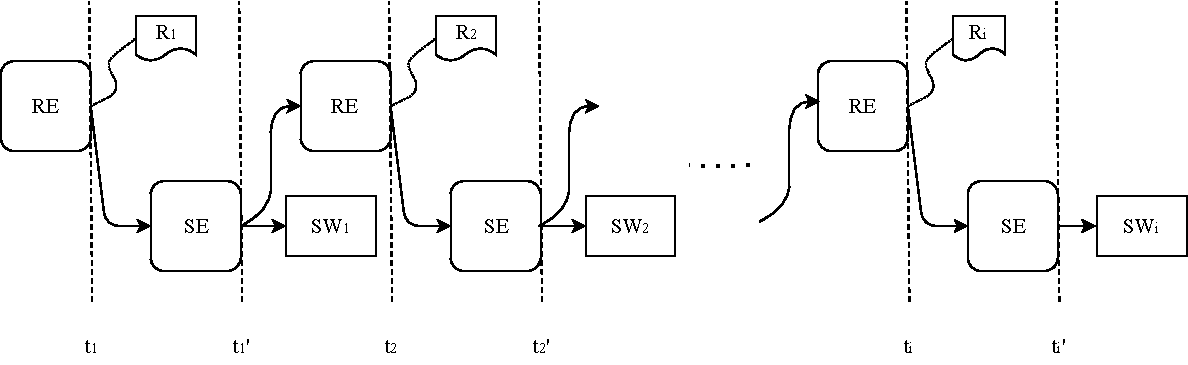
\includegraphics[width=0.8\textwidth,height=2in]{MetricsDiag.pdf}
	%\caption{Requirements engineering and development processes}
	%\label{fig:Metrics_shot}
%\end{figure}

%In these metrics we consider a maturity of requirements as a characteristic of the quality.
%
\autoref{fig:Metrics_shot} provides a graphical explanation of the metrics. The workflow is divided into requirements engineering (RE) 
and system implementation (SI) processes' iterations along the time line: $t_{1},t_{2},...,t_{m}$ - 
instants of time for RE phases (RE iteration); $t_{1}',t_{2}',...,t_{m}'$ - 
instants of time for implementation process based on the provided requirements (SI iteration).
The output of every RE iteration is RE artifact (a document with the full set of the requirements) - depicted as $R_{1},R_{2},...,R_{j}$; and every SI phase results into SI artifact, 
e.g., software architecture (shown as SW), till the end of the SI phase, which leads to the release of a product and end of the project. 

The input for the first iteration of RE process is a "raw" requirements. During the RE phase, the requirements become elaborated (changed with respect to a project's demands); the result of this process is a corrected RE artifact, that is an input 

\newpage
\hfill \break

\vspace{5.4cm}

to the next stage (SI). Therefore, we consider the initial RE artifact as a document \textit{$\mu(R_{j})=0$}. 
 
%\subsection{Metrics for a full set of requirements}

We defined, that every RE artifact has its index of maturity. The range of this metric varies from 0 to 1: 0 means ``bad'' and 1 indicates ``good'' quality.
The maturity index is inferred from a number of iterations (a certain amount of changes applied to requirements' document) and the time spent for RE and implementation process.
The more mature a requirement is, the less changes (iterations) the artifact requires, and the shorter the time for the development process. 
\textsl{Thus, the better quality of the requirements: the higher index of the requirements maturity} (\autoref{eqn:maturity_ind}). 

In \autoref{eqn:maturity_ind}, the maturity index reflects, how far the considered requirements with the certain maturity parameters (presented as a sum of the metrics for the full set of the requirements - $\sum\mu_{n}(R_{j})$) from their ``good'' state (defined as 1)

  \begin{equation}\label{eqn:maturity_ind}
\textrm{\textit{maturity index}} = \frac{1}{\sum_{i=1}^{n}\mu_{i}(R_{j})}
	\end{equation}

where $(R_{j}$) is a considered RE artifact; $j$ is an starting iteration for calculation.
%where $\mu(R_{j})$ is a calculated number of the iterations for a considered RE artifact $(R_{j}$); $j$ is an initial iteration for calculation.

Consequently, to calculate the \textit{maturity index} of the requirements, the following metrics should be determined:

 \begin{equation}\label{eqn:mu1}
\mu_{1}(R_{j}) = m-j
	\end{equation}
	
\textrm{end of the number of iterations for the requirements} $R_{j}$;

 \begin{equation}\label{eqn:mu2}
\mu_{2}(R_{j}) = t_{m}\acute{}-t_{j}    
 \end{equation}

\textrm{amount of time (in hours) between initial and the last phases of the development process applying the requirements} $R_{j}$;

%\begin{equation}\label{eqn:mu3}
%\mu_{3}(R_{j}) = \displaystyle\sum_{j} t_{j+1}-t_{j}\acute{}
%\end{equation}
%
%,\textrm{total amount of time (in hours) required for SI process};


%(here, along with requirements' maturity, we can also talk about such quality criterion as the requirements' comprehensibility);
%$\mu_{4} = \displaystyle\sum_{j} (t_{j+1}-t_{j}\acute{} + p_{j}*(t_{j}\acute{} - t_{j}))$

%\subsection{Metrics for a single requirement}



\subsection{Use Case for applying \cbc}
\label{sec:usecase} 

``Router'' use case exposes an example of a simple ``Router'' component with configured quality of service (QoS) management, which is used in telecommunication networks. In this use case Stakeholders have provided the system requirements (\autoref{tab:SR}) as a text document with semi-structured information and a simple component diagram (\autoref{fig:route}). 
\begin{figure}[!t]
\centering
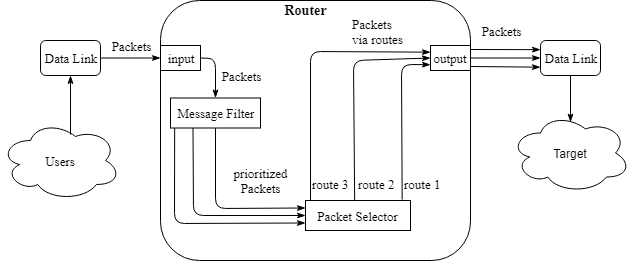
\includegraphics[width=3.5in]{use_case/router.png}
\caption{Diagram of the Router in the Network}
\label{fig:route}
\end{figure}

\begin{table}
	\centering
		\begin{tabular}{p{8cm}}
\small
\begin{center}
\textbf{\textit{System requirements.}}
\end{center}
``In communication system Data Link (DL) is usually used by several users. The users can proceed with different types of traffic. For better use of Data Link resources, traffic from diverse users can differ by priorities (depends on QoS and user's agreement). Depending on the priority, traffic should be forwarded along a certain route with a defined latency. For high priority packets the route shall be defined with the lowest latency. The lower priority of traffic, the higher latency the provided route has. Configuration input for Selector should be specified by QoS agreement of user.

Message Filter defines priority of packets and send them directly to Selector. 

Selector should:
\begin{itemize}
	\item receive packets from Message Filter;
  \item define a proper route, according to packet priority;
\end{itemize}

Packets shall be sent from Selector to Data Link using 3 routes.

All QoS policy is defined in Selector component. 

There are 3 data priorities: 
\begin{enumerate}
	\item High priority information - Selector should route such packets into 1st route only! 
  \item	Middle level priority - packets can be sent by Selector into 1st route , if the route is free; otherwise, traffic is transmitted into 2nd route;
  \item	Low priority - data can be sent in 3 routers, depends on which route is free at the moment.''
\end{enumerate}
\end{tabular}
	\caption{System Requirements Provided by Stakeholders}
	\label{tab:SR}
\end{table}

\normalsize 
\subsubsection{Requirements Structuring}
\label{sec:reqstruct}
Initial phase of development process is elicitation and analysis of requirements. We claim, that during analysis process \asp should be applied to the requirements in order to categorize them and form their structure. Considering further the ``Router'' use case, the following \asp can be assigned to the given requirements:\\

\small ``Req-1.	In communication system Data Link is usually used by several users.''

\normalsize[\textit{Mode aspect}] implies, that DL is in active state, when the users send traffic.\\

\small ``Req-2.	The users can proceed with different types of traffic.''

\normalsize [\textit{Signal aspect}] describes, that the packets have different types.\\

\small ``Req-3.	For better use of Data Link resources, traffic from diverse users can differ by priorities (depends on QoS in user's agreement).''

\normalsize [\textit{Signal aspect}] describes the traffic.\\

\small ``Req-4.	Depending on the priority, traffic should be forwarded along a certain route with a defined latency.'' 

\normalsize \begin{itemize}
	\item \textit{Parameter definition aspect} indicates, that priorities, routes and latency can be kept as re-useable parameters;
	\item \textit{Signal aspect} describes input for the routes;
	\item \textit{Functional aspect} describes the behavior of ``Packets Selector'';
	\item \textit{Temporal property aspect} shows, that the statement includes a condition;
\end{itemize}

The rest of the requirements should be analyzed and structured similarly.

After requirements have been categorized, the requirements engineer can proceed with the following inspection. First of all, he/she should check, if all requirements have \asp. Next, re-consider the requirements with more than 1 aspect in their categorization; it can mean, that such requirements are not precise enough. For example, the requirement ``Req-4'':\\

\small ``Req-4. Depending on the priority, traffic should be forwarded along a certain route with a defined latency.``

\normalsize
\begin{itemize}
	\item \textit{Parameter definition aspect}, 
	\item \textit{Signal aspect},
	\item \textit{Functional aspect}, 
	\item \textit{Temporal property aspect.}
\end{itemize}

It can be splitted into several requirements according to \asp categories:\\

For [\textit{Functional aspect}]:

\small
``Req-4.1.	 Selector should forward traffic along a certain route.''\\

\normalsize For [\textit{Parameter definition aspect}]:

\small
``Req-4.2.	 Every route operates with defined latency.''

``Req-4.3.	There are several (three) routes.''

``Req-4.4.	There are several priorities for traffic.''\\

\normalsize For [\textit{Signal aspect}]:

 \small ``Req-4.1.	Traffic is prioritized.''\\

\normalsize For [\textit{Temporal property aspect}]:

\small ``Req-4.2.	Traffic priority defines a route for traffic.''\\

\normalsize The ideal case is when every requirement has only one aspect, but in real project requirements categories usually overlap each other. Therefore, the number of \asp attached to a requirement should tend to be minimized.

After applying this method also to the other requirements, we have obtained the following structure of requirement, presented in \autoref{tab:structuredHLR}.

\begin{table*}
	\centering
		\begin{tabular}{| p{11cm}  | p{6cm} |}
			\small ``Req-1.	 In communication system Data Link is usually used by several users.'' &	[\textit{Mode aspect}]\\
``Req-2.	The users can proceed with different types of traffic.'' & [\textit{Signal aspect}]\\	
``Req-3.	For better use of Data Link resources, traffic from diverse users can differ by priorities (depends on QoS in user's agreement).'' & [\textit{Signal aspect}] \\
``Req-4.1	 Selector should forward traffic along a certain route.''& [\textit{Functional aspect}]\\ 
``Req-4.2	Every route operates with defined latency.'' & [\textit{Parameter definition aspect}]\\		
``Req-4.3	There are several (three) routes.'' & [\textit{Parameter definition aspect}] \\
``Req-4.4 There are several priorities for traffic.'' & [\textit{Parameter definition aspect}]\\
``Req-4.5	Traffic is prioritized.'' & [\textit{Signal aspect}] \\
``Req-4.6	Traffic priority defines a route for traffic.'' & [\textit{Temporal property aspect}] 	\\
``Req-5.	For high priority packets the route shall be defined with the lowest latency.'' & [\textit{Temporal property aspect}] \\
``Req-6.	The lower priority of traffic, the higher latency the provided route has.'' & [\textit{Temporal property aspect}] \\
``Req-7.	Configuration input for Selector should be specified by QoS agreement of user.'' & [\textit{Signal aspect}] \\
``Req-8.1	Message Filter defines priority of packets.'' & [\textit{Functional aspect}] \\	
``Req-8.2 Message Filter sends packets directly to Selector.'' &  [\textit{Functional aspect}] \\
``Req-9.1	Selector should receive packets from Message Filter.'' & [\textit{Functional aspect}] \\
``Req-9.2	Selector should define a proper route, according to packet priority.'' & [\textit{Functional aspect and Temporal property aspect}]\\
``Req-10.1	Selector shall send packets to Data Link.'' & [\textit{Functional aspect and Signal aspect}] \\
``Req-10.2	Selector shall use 3 routes for packets sending to Data Link.'' & [\textit{Functional aspect}] \\
``Req-10.3	There are 3 routes for sending packets from Selector to Data Link.'' & [\textit{Parameter definition aspect}] \\
``Req-11	All QoS policy is defined in Selector component.'' & [\textit{Functional aspect}] \\
``Req-12.1	There are 3 data priorities.'' & [\textit{Parameter definition aspect}] \\
``Req-12.2.	High priority information - Selector should route such packets into 1st route only!'' & 
[\textit{Temporal property aspect}] \\
``Req-12.3.	Middle level priority - packets can be sent by Selector into 1st route , if the route is free; otherwise, traffic is transmitted into 2nd route.'' & [\textit{Temporal property aspect}] \\
``Req-12.4.	Low priority - data can be sent in 3 routers, depends on which route is free at the moment.'' & [\textit{Temporal property aspect}] \\
		\end{tabular}
	\caption{Structured Requirements with Attached Aspects}
	\label{tab:structuredHLR}
\end{table*}

\normalsize
Now we have more consistent high-level requirements (HLR) in comparison with the requirements initially provided by the stakeholder. That means, the requirements are better structured, more precise and less complex. These characteristics rise quality of the requirements. Therefore, it is easier to work with such requirements during development phase or review process.

These structured HLR now can be an input for system design process. Developers can also analyze the requirements and provide additional requirements, which were inferred from HLR. For this purpose, there exists a \textit{Design Choice aspect}. This aspect indicates, that changes in requirements have been done by developers team. Example of such requirement is provided:

\small''Req-13.  Packets follow the Ethernet standard.''

\normalsize the requirement now has two \asp [\textit{Signal aspect} and \textit{\textbf{Design Choice aspect}}]. 


\normalsize \subsubsection{Requirements Review}
\textit{Aspects} support also requirements review process. Every \textit{aspect} provides a check-list specified for respective category of requirement. This feature serves for more rigorous review of the requirements instead of a general check. More over, different \asp imply different activities of requirements checking. As an example from the use case, to inspect Req-10.2: \\

\small ``Req-10.2.  Selector shall use 3 routes for packets sending to Data Link.'' 

\normalsize [\textit{Functional aspect}], here reviewer checks correctness of algorithms implemented within this requirement. However, the same check is useless for Req-4.3: \\

\small ``Req-4.3.  There are several (three) routes.'' 

\normalsize ,which is defined by [\textit{Parameter definition aspect}].\\

Working with HLR structured by \asp, the reviewer can trigger the following revision:
\begin{itemize}
	\item whether \textit{aspects} have been applied to each requirement,
  \item whether the \textit{aspects} match appropriately with the considered requirements (the reviewer can propose additional \asp or make changes in the ones already attached),
	\item whether all \asp check-lists give successful outcomes.
\end{itemize}

%\input{review}
\section{Evaluation and Validation}
\label{eval}
Firstly, \cbc has been validated by industry use case within ASSET project during avionics component development. 
%The outcames of this  – what impact the Aspects make on requirements reviewing process – handle requirements complexity.

Next step for evaluation and validation of \cbc can be series of empirical studies conducting with students, at Fortiss research institute to find out, how a user can handle unstructured system requirements applying \cbc and without \cc. The outcomes will be compared in order to check, whether quality of the considered requirements increases with \cc application. For this purpose criteria of comparison can be defined as:
\begin{itemize}
	\item time-consumption during system development based on the structured and unstructured requirements
	\item comprehension of the structured and unstructured requirements (e.g. time for read and understanding requirements)
	\item number and types of errors have been corrected within reviewing process
\end{itemize}

However, these criteria can vary depending on further results of study.

\section{Related Work}
\label{sec:relatedwork} 

\subsection{What does ``quality'' mean?}

Despite multiple publications about requirements quality and its assessment, 
the term ``quality'' is still subjective~\cite{Mund:2017},~\cite{Femmer:2017}. 
Industry standards~\cite{ISO/IEC/IEEE:2011} specify characteristics and criteria, 
which presumed effective for improving requirements quality, e.g, completeness, unambiguity. 
Additionally, the research community provided several types of quality definition and methods for its assessment. 
For example, Lamsweerde provides a defect-based checklist to inspect requirements for possible flaws 
and errors in ~\cite{Lamsweerde:2009}; Pohl proposes a framework defining dimensions of quality: 
the specification dimension, the representation dimension, the agreement dimension~\cite{POHL:1994}.
This approach considers such imprecise and subjective attributes as requirements adequacy or pertinence, thereby purporting uncertain assessment.
Instead of analyzing the meaning of the requirements, our method takes into account a maturity of the whole requirements artifact (RA).

%This approach purports an uncertain assessment due to impreciseness of the considered attributes, 
%such as requirements adequacy or pertinence. Instead of such level of granularity for requirements 
%consideration, our method take into account a requirements artifact (RA) in general. 

Another approach implies syntactic check of the requirements text for improving its comprehension, 
correctness, ambiguity and other akin characteristics e.g.~\cite{Ferrari:2014},~\cite{Berry:2006}.
All these metrics apply intrinsic inspection of requirements and assess qualitatively the requirements' statement. 
In contrary, our metrics provide a \textit{quantitative} analysis of a full document with the requirements.

In comparison with methods described above, activity-based quality models shift their approach from inherent properties of the requirements 
to the context of process, and propose a meta quality model~\cite{Wagner:2012},~\cite{Femmer:2015}. 
Furthermore, the "quality question" also turns to a consideration of how the requirements quality impacts the project success and the relation between 
them in scientific community~\cite{Emam:1995},~\cite{Kamata:2007}, so as among practitioners~\cite{BeattyHokanson:2014}.
In contrast to the approaches, our metrics grant a quick and lightweight method for the quality assessment considering the number of the requirements' corrections.
%our metrics grant a relative simplicity level and provide a precision with cardinal number in assessment.

%Pleiad 
A series of studies about the relation between quality and project outcomes, ~\cite{Verner:2005},~\cite{Kamata:2007},~\cite{Noorwali:2015} triggers our research to the proposed metrics. Scientific papers investigating maturity of requirements~\cite{Basili:1981},~\cite{FARBEY:1990} and their complexity~\cite{Antinyan:2016} give a base for the idea of transforming a relation between requirements quality and number of changes in requirements document into quantitative measurement, but they described the quality aspects within the ongoing process. The metrics presented in this paper consider a requirements artifact as a ``black box'' for its maturity and a process of adjusting the requirements at RE and implementation phases, in a quantitative way, once a project is over.

%Now exists a vast majority of quality definitions:
%\begin{enumerate}
	%\item in industry Standards - set of attributes such as completeness, unambiguity... [ISO/IEC/IEEE-29148];
	%\item in scientific point of view, [Lamsweerde] gives a general list of characteristics, [Pohl] proposed a framework defining dimensions of quality (• the specification dimension, • the representation dimension, the agreement dimension.);
	%\item check requirements language for lacking of errors, defects, ambiguity and possible reasons for incomprehension [];
	%\item different kind of quality models such as activity-based[10], natural-language requirements specifications[7] %(activity, stupid!)
%\end{enumerate}
%
%
%\subsection{Metrics for quality measure}
%\begin{itemize}
	%\item methodology for context-specific RE artifact quality measuring has in its base an activity-based quality model [activity, stupid!] - brief description
	%\item the mentioned attributes should be satisfied 
	%\item some researchers shift their look to product quality measurement e.g [measuring success], however 
%\end{itemize}
%
%All these metrics intend to intrinsic inspection of requirements. In contrast to them, we propose the quantitative metrics for assessment of requirements quality
%\section{ExpectedContributions}
Conducting this research the following goals will be achieved:
\begin{itemize}
\item	to bridge a gap between requirements engineers and reviewers providing to them a feasible method based on requirements \textit{aspects}, which guides both roles within requirements reviewing process and supports a communication flow between these two roles. That leads to ease of redundancy in the work-flow,
\item	to close a gap between requirements reviewer and system developers by providing a structured constitution of requirements which is in help to concentrate a precise overview on the requirements (as on a whole scope of them so as only on specific category of requirements or part of them, depending on categorization granularity). As a result, a reviewer can provide a more specified and detailed response to developers on any changes in a system,
\item	moreover, \textit{aspects} concept links a bridge between requirements engineers and developers, so that a structure of \textit{aspects} itself includes key “hints” for every requirements category, which help in seamlessly mapping requirements into design of a system,
\item	the \textit{aspects} is a general concept, which can be applied independently on a specific tool chain. They can be simply applied with a familiar development tool. It gives a flexibility in use and reduces the cost for new tools learning,
\item	semi-automatically check-lists, which are an extensions for every aspect, useful for making a requirements review easier and, consequently, less time- and resource-consuming.
\end{itemize}
All in all, the \textit{aspects} concept provides a common instrument for all mentioned above roles (requirements engineers, reviewers, developers). All these points can increase a quality of requirements and thereby, save a significant amount of resources in system development such as project time and expenses.

\section{Current Status}
At the moment, the research goes further with the idea of \cbc. It implies to consider an impact of \cc on a whole development process including testing phase. Also the study is supposed to cover requirements reuse and a role of the \cbc in supporting that process.

Currently, question of relevant and sufficient methods for proper evaluation of the \cbc still arises. The investigation of possible techniques is in process.


%considers relevant and sufficient methods for proper evaluation of the \cbc. Simultaneously to this research task, further implementation of the \asp concept in \af tool and its testing continues. Moreover, the study is supposed to consider an impact of the \cbc on other phases of development process, such as system testing, requirements reuse and etc.

%Next steps within the research appear as a checking of usability of the concept conducting a series of empirical experiments.


%Implemented within the MIRA framework \cite{18MIRA} in \autof and reflecting requirements engineering activities form the initial stage of a development process, the \textit{aspects} can represent a general concept supporting its unique method, which may be applied within other tools thereby, providing tool\textbackslash platform- independence. The next pace in this direction of the research is a deeper investigation of this theory and its consideration on practice.
%
%And the most challenging question about proper and adequate validation technics for the Aspects concept will be considered in future work in this study.

% no \IEEEPARstart


% You must have at least 2 lines in the paragraph with the drop letter
% (should never be an issue)


%\hfill 
% 
%\hfill 
%
%\subsection{Subsection Heading Here}
%Subsection text here.
%
%
%\subsubsection{Subsubsection Heading Here}
%Subsubsection text here.


% An example of a floating figure using the graphicx package.
% Note that \label must occur AFTER (or within) \caption.
% For figures, \caption should occur after the \includegraphics.
% Note that IEEEtran v1.7 and later has special internal code that
% is designed to preserve the operation of \label within \caption
% even when the captionsoff option is in effect. However, because
% of issues like this, it may be the safest practice to put all your
% \label just after \caption rather than within \caption{}.
%
% Reminder: the "draftcls" or "draftclsnofoot", not "draft", class
% option should be used if it is desired that the figures are to be
% displayed while in draft mode.
%
%\begin{figure}[!t]
%\centering
%\includegraphics[width=2.5in]{myfigure}
% where an .eps filename suffix will be assumed under latex, 
% and a .pdf suffix will be assumed for pdflatex; or what has been declared
% via \DeclareGraphicsExtensions.
%\caption{Simulation results for the network.}
%\label{fig_sim}
%\end{figure}

% Note that the IEEE typically puts floats only at the top, even when this
% results in a large percentage of a column being occupied by floats.


% An example of a double column floating figure using two subfigures.
% (The subfig.sty package must be loaded for this to work.)
% The subfigure \label commands are set within each subfloat command,
% and the \label for the overall figure must come after \caption.
% \hfil is used as a separator to get equal spacing.
% Watch out that the combined width of all the subfigures on a 
% line do not exceed the text width or a line break will occur.
%
%\begin{figure*}[!t]
%\centering
%\subfloat[Case I]{\includegraphics[width=2.5in]{box}%
%\label{fig_first_case}}
%\hfil
%\subfloat[Case II]{\includegraphics[width=2.5in]{box}%
%\label{fig_second_case}}
%\caption{Simulation results for the network.}
%\label{fig_sim}
%\end{figure*}
%
% Note that often IEEE papers with subfigures do not employ subfigure
% captions (using the optional argument to \subfloat[]), but instead will
% reference/describe all of them (a), (b), etc., within the main caption.
% Be aware that for subfig.sty to generate the (a), (b), etc., subfigure
% labels, the optional argument to \subfloat must be present. If a
% subcaption is not desired, just leave its contents blank,
% e.g., \subfloat[].


% An example of a floating table. Note that, for IEEE style tables, the
% \caption command should come BEFORE the table and, given that table
% captions serve much like titles, are usually capitalized except for words
% such as a, an, and, as, at, but, by, for, in, nor, of, on, or, the, to
% and up, which are usually not capitalized unless they are the first or
% last word of the caption. Table text will default to \footnotesize as
% the IEEE normally uses this smaller font for tables.
% The \label must come after \caption as always.
%
%\begin{table}[!t]
%% increase table row spacing, adjust to taste
%\renewcommand{\arraystretch}{1.3}
% if using array.sty, it might be a good idea to tweak the value of
% \extrarowheight as needed to properly center the text within the cells
%\caption{An Example of a Table}
%\label{table_example}
%\centering
%% Some packages, such as MDW tools, offer better commands for making tables
%% than the plain LaTeX2e tabular which is used here.
%\begin{tabular}{|c||c|}
%\hline
%One & Two\\
%\hline
%Three & Four\\
%\hline
%\end{tabular}
%\end{table}


% Note that the IEEE does not put floats in the very first column
% - or typically anywhere on the first page for that matter. Also,
% in-text middle ("here") positioning is typically not used, but it
% is allowed and encouraged for Computer Society conferences (but
% not Computer Society journals). Most IEEE journals/conferences use
% top floats exclusively. 
% Note that, LaTeX2e, unlike IEEE journals/conferences, places
% footnotes above bottom floats. This can be corrected via the
% \fnbelowfloat command of the stfloats package.




%\section{Conclusion}
%The conclusion goes here.




% conference papers do not normally have an appendix


% use section* for acknowledgment
%\section*{Acknowledgment}
%
%
%The authors would like to thank...





% trigger a \newpage just before the given reference
% number - used to balance the columns on the last page
% adjust value as needed - may need to be readjusted if
% the document is modified later
%\IEEEtriggeratref{8}
% The "triggered" command can be changed if desired:
%\IEEEtriggercmd{\enlargethispage{-5in}}

% references section

% can use a bibliography generated by BibTeX as a .bbl file
% BibTeX documentation can be easily obtained at:
% http://mirror.ctan.org/biblio/bibtex/contrib/doc/
% The IEEEtran BibTeX style support page is at:
% http://www.michaelshell.org/tex/ieeetran/bibtex/
\bibliographystyle{IEEEtran}
% argument is your BibTeX string definitions and bibliography database(s)
\bibliography{AspectsBib}
%
% <OR> manually copy in the resultant .bbl file
% set second argument of \begin to the number of references
% (used to reserve space for the reference number labels box)

%\begin{thebibliography}{19}
%%
%%%\bibitem{IEEEhowto:kopka}
%%%H.~Kopka and P.~W. Daly, \emph{A Guide to \LaTeX}, 3rd~ed.\hskip 1em plus
%%%  0.5em minus 0.4em\relax Harlow, England: Addison-Wesley, 1999.
%%
%\bibitem{1Review} A Review of Requirement Engineering Issues and Challenges in Various Software Development Methods
%\bibitem{2Pohl}	Pohl, 2010; 
%\bibitem{3Eckhardt}	Jonas Eckhardt. “Categorizations of Product-related Requirements in Practice Observations and Improvements”
%\bibitem{4Robertson}	Robertson and Robertson,2012; 
%\bibitem{5Sommerville} Sommerville and Kotonya, 1998;
%\bibitem{6Lamsweerde}	Van Lamsweerde, A. (2001). Goal-oriented requirements engineering: A guided tour. In
%Proceedings of the 5th International Symposium on Require-ments Engineering (RE),
%\bibitem{7DO-178C}	DO-178C.
%\bibitem{8DO-331}	DO-331
%\bibitem{9ISO29148}	ISO29148:2011
%\bibitem{10Broy}	 Broy, M. (2016). Rethinking Nonfunctional Software Requirements: A Novel Approach Categorizing System and Software Requirements. In Hinchey, M., editor, Software Technology: 10 Years of Innovation in IEEE Computer. John Wiley \& Sons/IEEE Press.
%\bibitem{11Mager}	 Mager, P. (2015). Towards a Profound Understanding of Non-Functional Requirements. Master’s thesis, Tech-nische Universität München.
%\bibitem{12RQS}	Requirement Quality Suite 
%\bibitem{13EARS}	EARS
%\bibitem{14UML}	UML 
%\bibitem{15Goals}	“Does Goal-Oriented Requirements Engineering Achieve its Goal?”, Tuefl, Eckardt, Mund, Femmer
%\bibitem{16NaPiRe}	Supporting Requirements-Engineering Research That Industry Needs. The NaPiRE Initiative” by Daniel Mén-dez Fernández
%\bibitem{17MiniDuide}	Mini-Guideline to Requirements Engineering. Birgit Penzenstadler
%\bibitem{18MIRA}	 MIRA framework
%\bibitem{4citation} B.H.C. Cheng and J.M. Atlee, “Research Directions in Requirements Engineering,” Proc. 2007 Future of Software Eng. (FOSE 07), 2007, pp.285–303.
%
%
%\end{thebibliography}

% that's all folks
\end{document}


